\PassOptionsToPackage{unicode=true}{hyperref}
\documentclass[aspectratio=169]{beamer} % 1610, 149, 54, 43 and 32
%\documentclass[aspectratio=43]{beamer} % 1610, 149, 54, 43 and 32

\usepackage{fontspec}
\usepackage{fancyvrb, fvextra}
\usepackage{xcolor, graphicx}

% multilingual support
\usepackage{polyglossia}
\setdefaultlanguage{polish} % by default polish settings and names
                            % only this, NOT \RequirePackage{polski} NOR \RequirePackage[polish]{babel}
\setotherlanguages{english} % provide english language option too (for code printing)

\usepackage[ampersand]{easylist}

\usepackage{tikz}
\usetikzlibrary{positioning} % for positionig nodes with `right = of X`
\usetikzlibrary{arrows.meta, decorations.markings} % for arrows formating in tikzpicture
\usetikzlibrary{shapes} % for elipse nodes

\usetheme{CambridgeUS}
\usecolortheme{dolphin}
%\usetheme{Rochester}
\setbeamertemplate{navigation symbols}{}
\xdefinecolor{icmgreen}{rgb}{0,0.55,0.46}
\usecolortheme[named=icmgreen]{structure}

\title[Monitoring w obiektach DC]{Budowa systemu monitoringu infrastruktury obiektów data center}
\author[Robert Paciorek]{Robert Paciorek\\{\footnotesize <rrp@icm.edu.pl>}}
\date{Warszawa 2020-02-27}
\institute[ICM UW]{Interdyscyplinarne Centrum Modelowania Matematycznego i Komputerowego,\\Uniwersytet Warszawski}
\titlegraphic{
\includegraphics[height=1.2cm]{monitoring_obiektow_data_center-img/logo_icm}\hspace*{3cm}~
\includegraphics[height=1.2cm]{monitoring_obiektow_data_center-img/logo_uw}}

\begin{document}

\begin{frame}
\titlepage
\end{frame}

\section{ICM UW}

\begin{frame}[fragile]
\begin{easylist}[itemize]
& jednostka pozawydziałowa Uniwersytetu Warszawskiego utworzona w 1993 roku
& ośrodek obliczeniowy – jedno z 5ciu polskich Centrum Komputerów Dużej Mocy
& meteo.pl, ftp.icm.edu.pl, wbn.edu.pl
& organizator międzynarodowej konferencji Supercomputing Frontiers Europe
&& najbliższa edycja 23 – 26 marzec 2020
\end{easylist}
\begin{center}
\includegraphics[height=2.2cm]{monitoring_obiektow_data_center-img/logo_scfe}\end{center}
\end{frame}

\section{Co monitorujemy w obiektach typu data center?}
\begin{frame}[fragile]
\begin{easylist}[itemize]
	& parametry środowiskowe w pomieszczeniach IT
	& działanie elementów systemu zasilania i chłodzenia
	& systemy bezpieczeństwa
		&& p.poż. (SSP, WDD, SUG)
		&& SSWiN
		&& KD
		&& CCTV
		&& detekcja zalania
	& zasilanie na poziomie szafy rack (per PDU / per gniazdko)
	& serwery i urządzenia sieciowe
\end{easylist}
\end{frame}

\section{Jak można budować system monitoringu?}
\begin{frame}[fragile]
\begin{easylist}[itemize]
	& niezintegrowane rozwiązania od dostawców poszczególnych podsystemów
	& systemy integrujące:
		&& Building Management System
		&& Security Management System
		&& Supervisory Control And Data Acquisition
		&& Data Center Infrastructure Management (software)
	& network (and servers) monitoring (Nagios, Zabbix, Grafana, ...)
	& rozwiązania dedykowane
\end{easylist}
\end{frame}

\begin{frame}[fragile]
\begin{easylist}[itemize]
	& jeden „supersystem” czy kilka specjalizowanych systemów?
		&& co lepsze?
		&& jaki podział?
			&&& IT, infrastruktura, bezpieczeństwo, ...
			&&& system nadrzędny pokazujący tylko krytyczne parametry z innych systemów
		&& od czego zależy?
	& funkcje systemu
		&& wizualizacja
		&& alarmy i powiadomienia
		&& archiwizacja danych
			&&& analiza „po zdarzeniowa”
			&&& statystyki i planowanie rozwoju
\end{easylist}
\end{frame}


\section{Integracja - wyciąganie informacji z innych systemów}
\begin{frame}[fragile]
\begin{easylist}[itemize]
	& twardo-drutowo czy protokolarnie?
	& TCP/IP
	& otwarte protokoły
	& bramkowanie
	& ograniczenia w dostępności informacji („system nie wystawia ...”)
\end{easylist}
\end{frame}


\section{Tworzenie systemu monitoringu na przykładzie rozwiązań w CT ICM}

\subsection{Obiekt}

\begin{frame}[fragile]
\begin{center}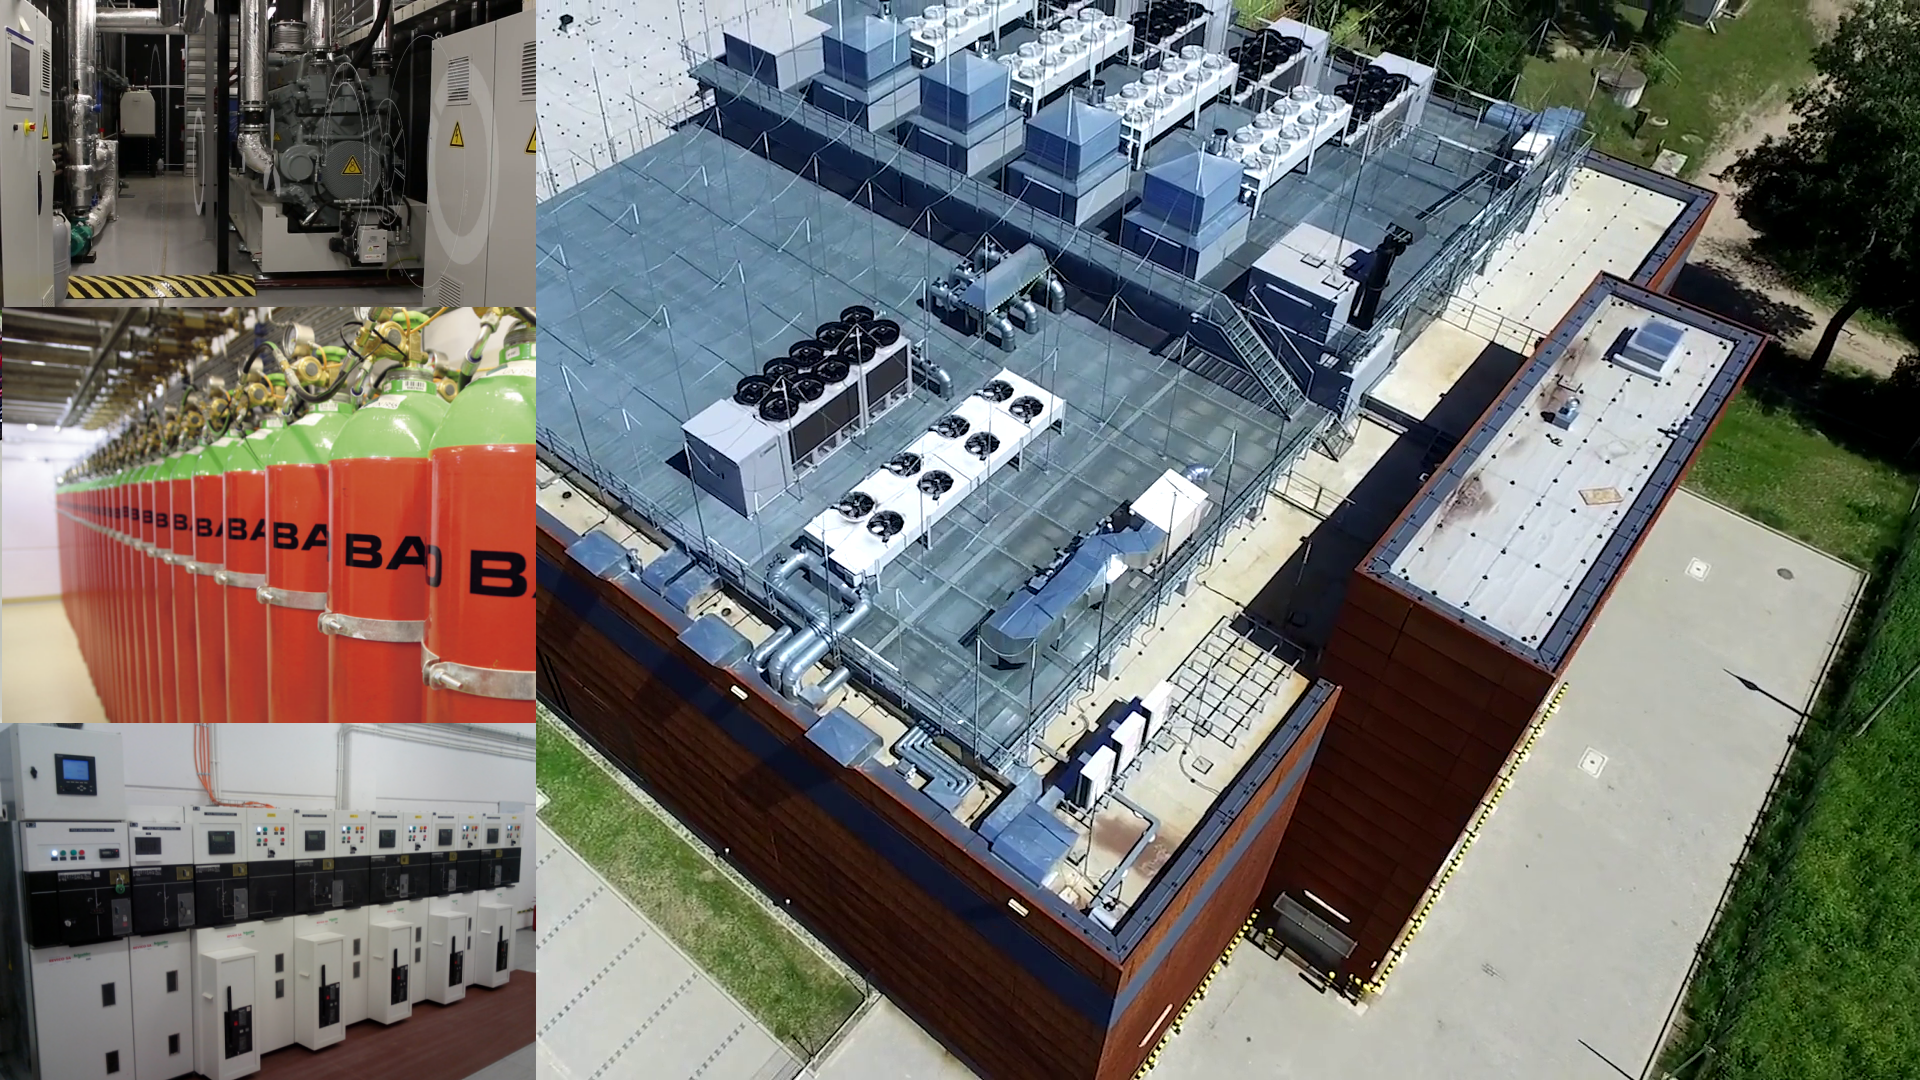
\includegraphics[width=.8\textwidth]{monitoring_obiektow_data_center-img/monitoring_dc-ct_icm}\end{center}
\end{frame}

\subsection{Założenia}
\begin{frame}[fragile]
\begin{easylist}[itemize]
	& dostosowany do naszych potrzeb system budujemy samodzielnie
	& system obejmuje całość monitoringu infrastruktury i systemów bezpieczeństwa
	& integracja oparta o warstwę TCP/IP
		&& wydzielona sieć fizyczna z kilkoma VLANami
		&& połączenia między modułami (węzłami sieci) światłowodowe
		&& redundancja połączeń
	& konwersja sygnałów trwardo-drutowych, RS485, itp na TCP/IP możliwie blisko źródła (w ramach „modułu”)
	& od dostawców wymagamy udostępniania wszystkich monitorowanych parametrów poprzez standardowe otwarte protokoły (modbus, BACnet, SNMP, ...) i pełnej dokumentacji tej komunikacji (wykazy rejestrów, pliki MIB, ...)
\end{easylist}
\end{frame}

\subsection{Szafki „automatyki”}
\begin{frame}[fragile]
\begin{center}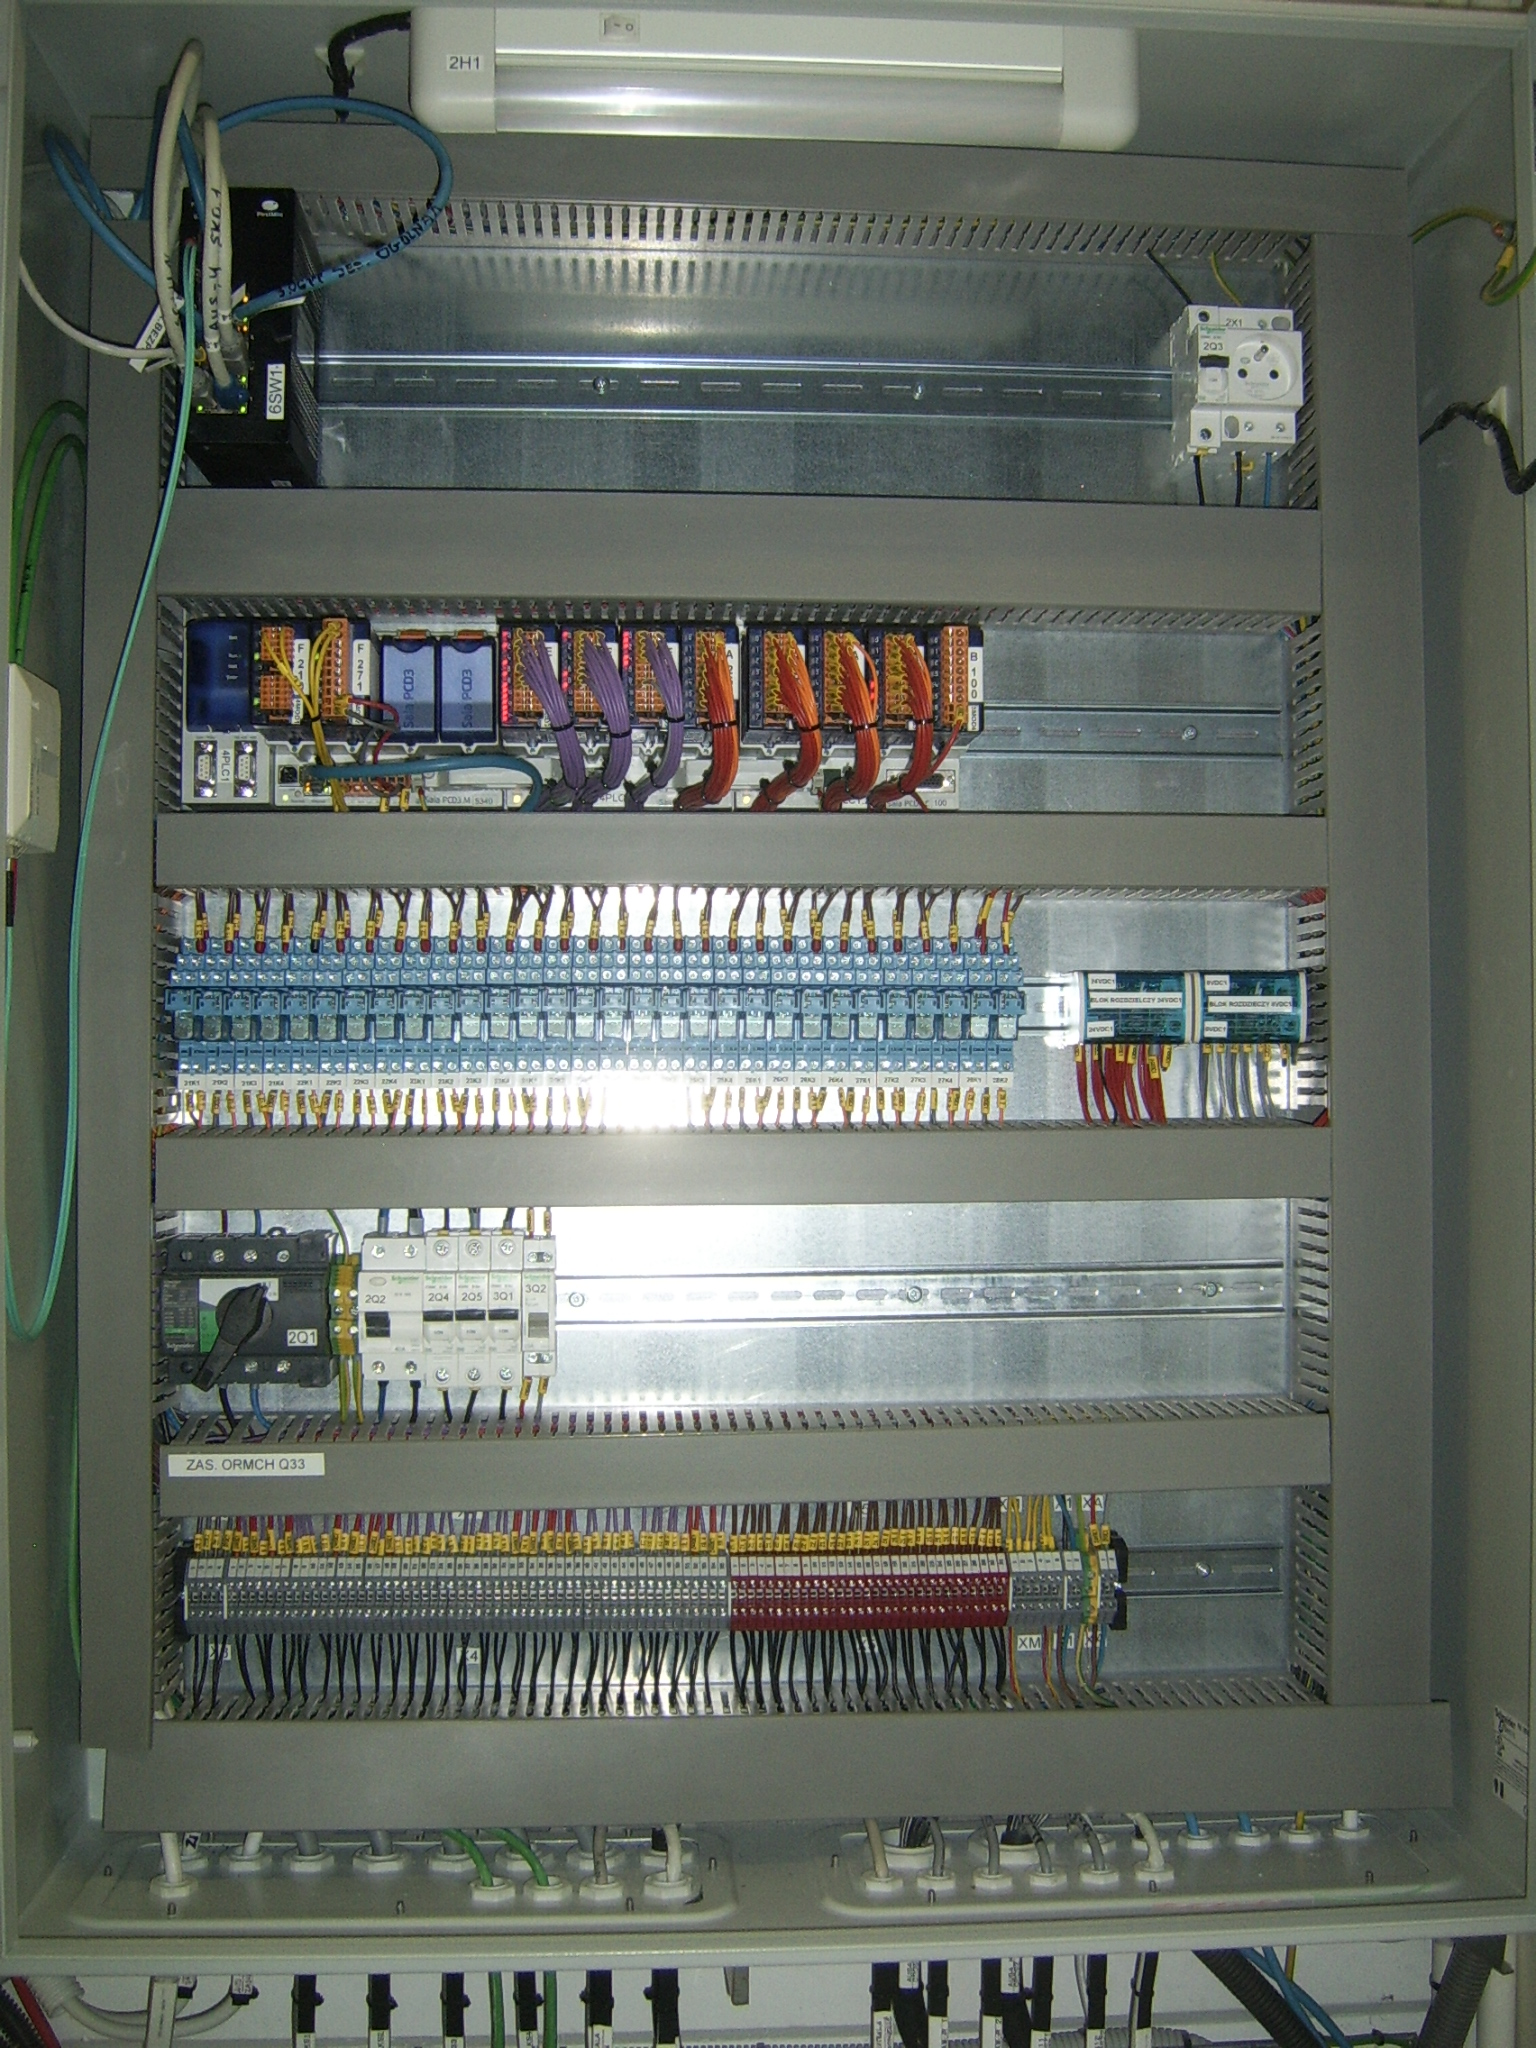
\includegraphics[width=.36\textwidth]{monitoring_obiektow_data_center-img/monitoring_dc-AUS}\hspace{.1\textwidth}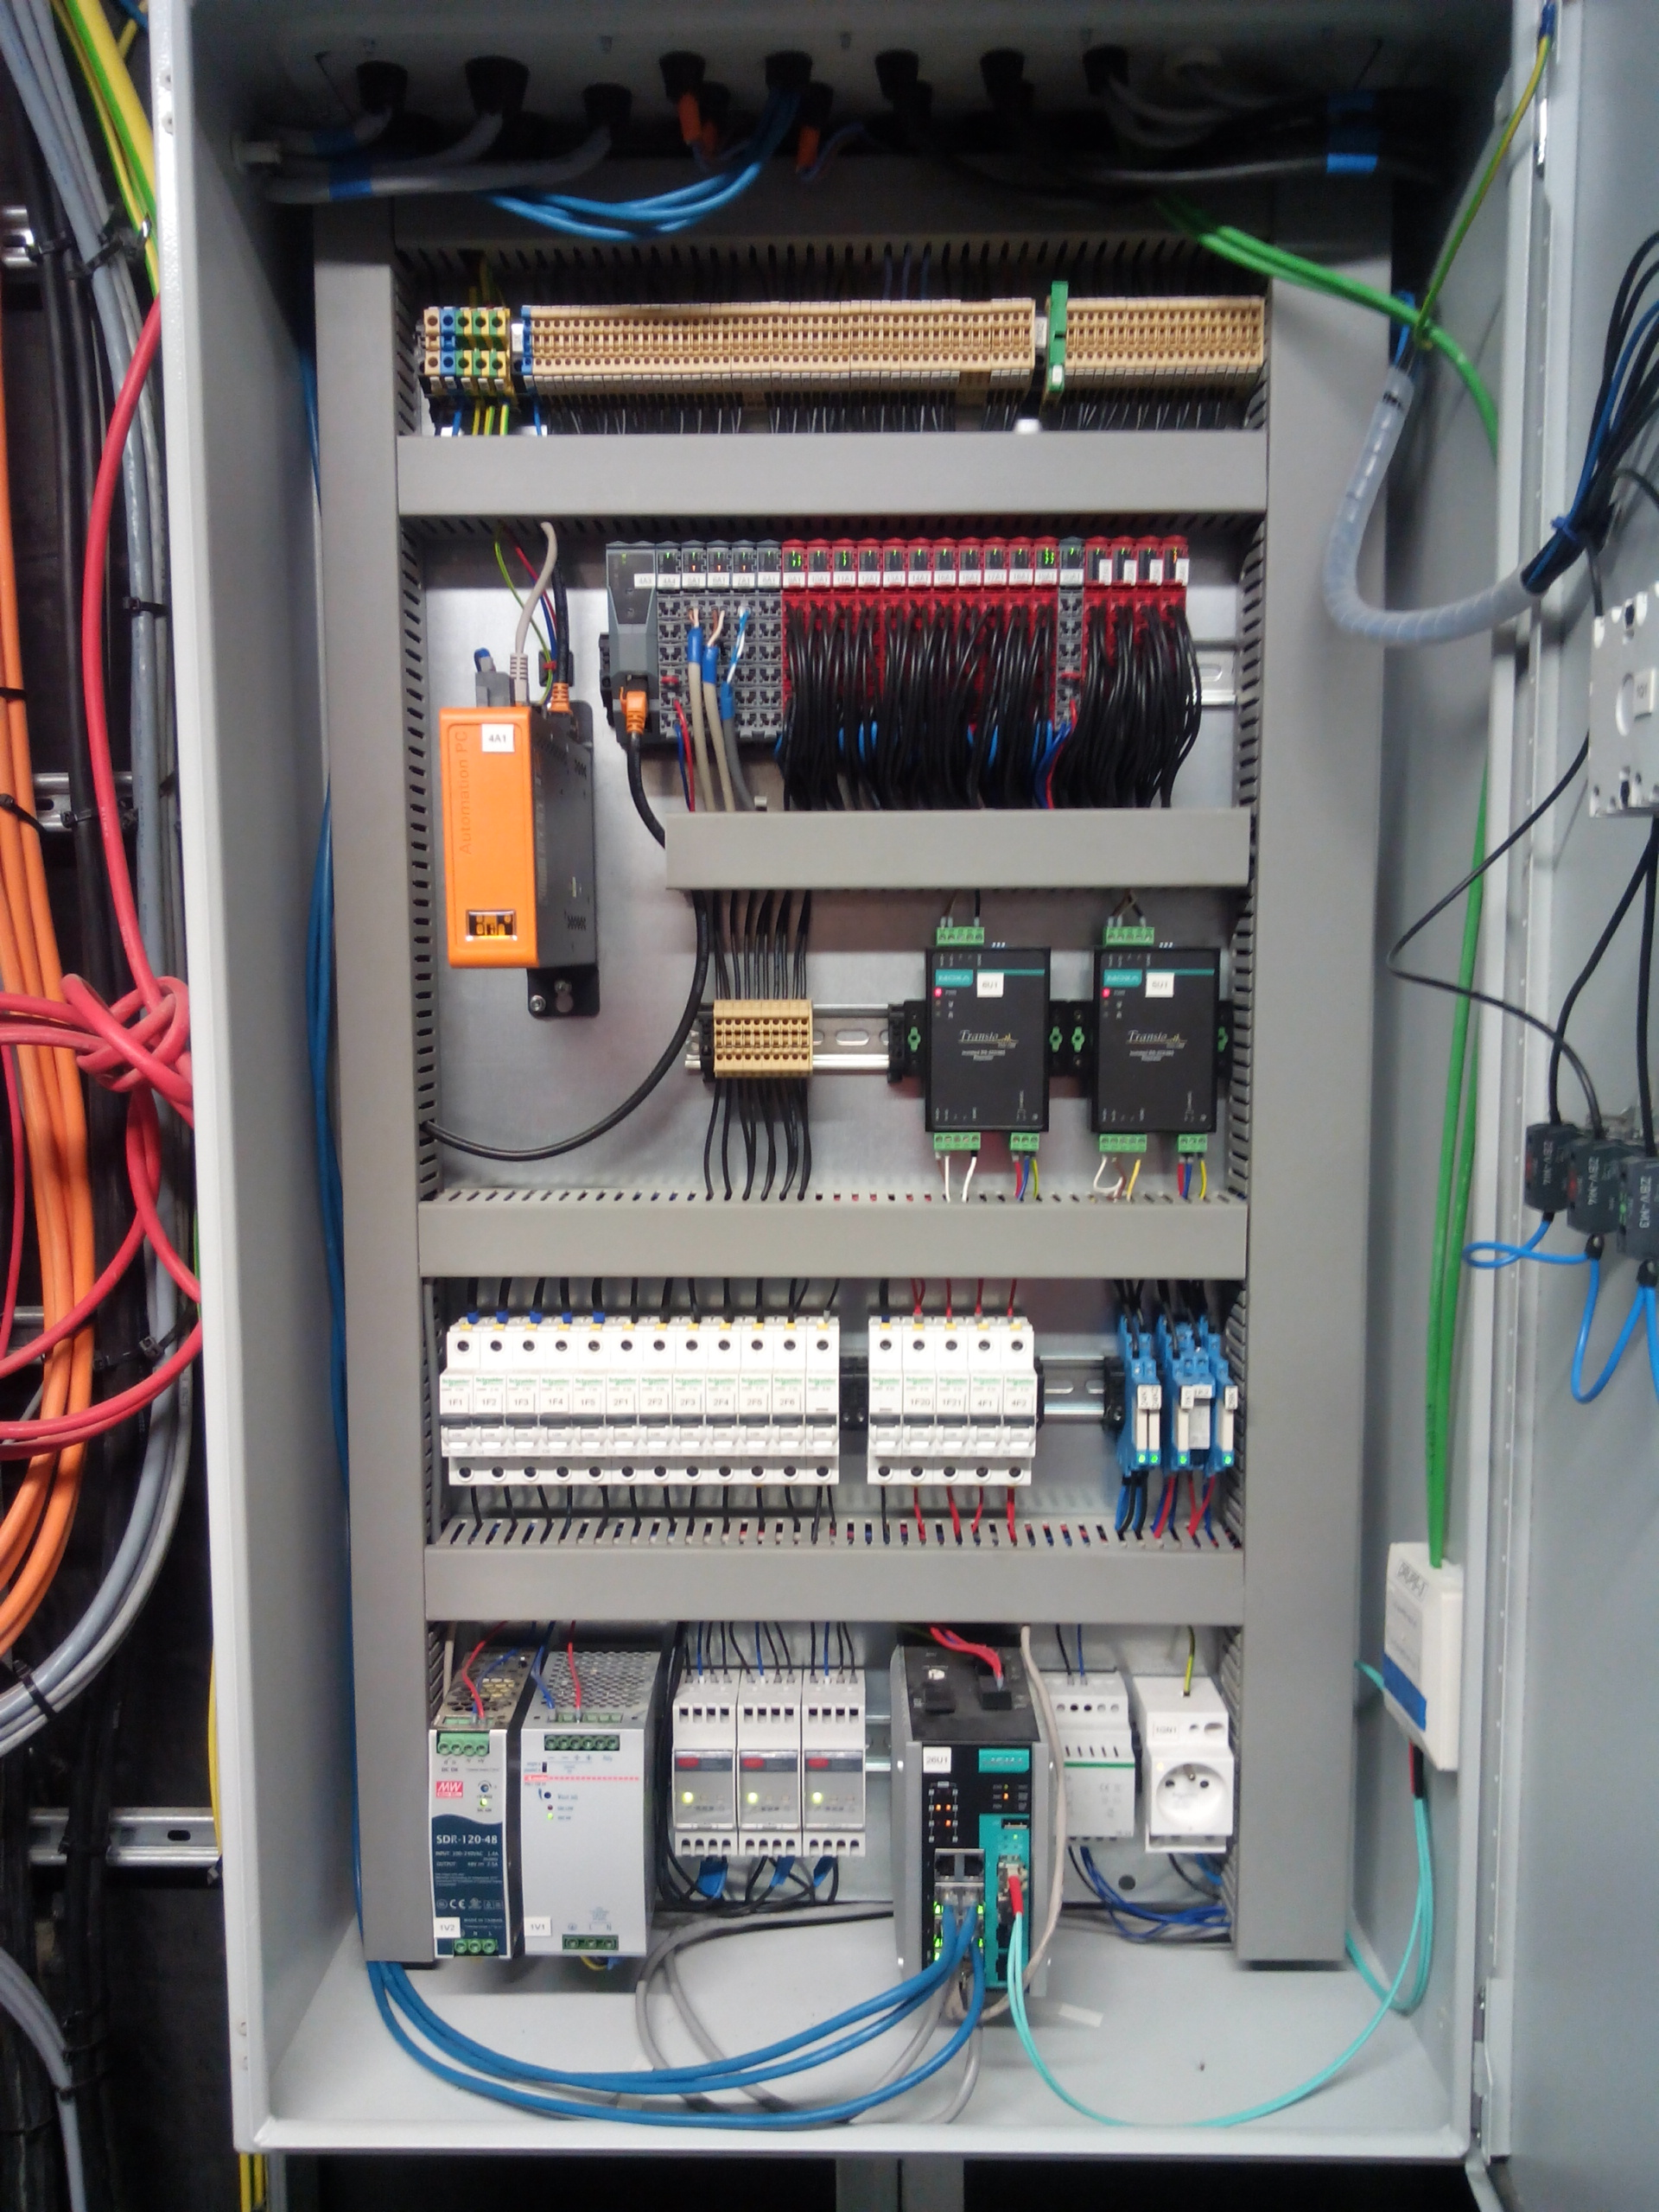
\includegraphics[width=.36\textwidth]{monitoring_obiektow_data_center-img/monitoring_dc-RMON}\end{center}
\end{frame}


\subsection{Realizacja systemu integracyjnego}
\begin{frame}[fragile]
\begin{easylist}[itemize]
	& rozwiązanie „ze świata informatyki”
	& zbieranie danych realizowane poprzez serwer Zabbix
		&& własne oprogramowanie do odczytu danych modbus i BACnet, oparte o:
			&&& BACnet Stack (\url{http://bacnet.sourceforge.net/})
			&&& libmodbus (\url{https://libmodbus.org/})
			&&& \Verb#crontab# i \Verb#zabbix_sender#
		&& dane trzymane w bazie MariaDB (MySQL)
			&&& zewnętrzny dostęp do danych
	& wizualizacja oparta o grafiki SVG
		&& JS użyty do podmiany wartości pól tekstowych w SVG
		&& PHP użyty do pobierania danych z bazy SQL dla JS
\end{easylist}
\end{frame}

\subsection{Wizualizacja - energetyka}
\begin{frame}[fragile]
\begin{center}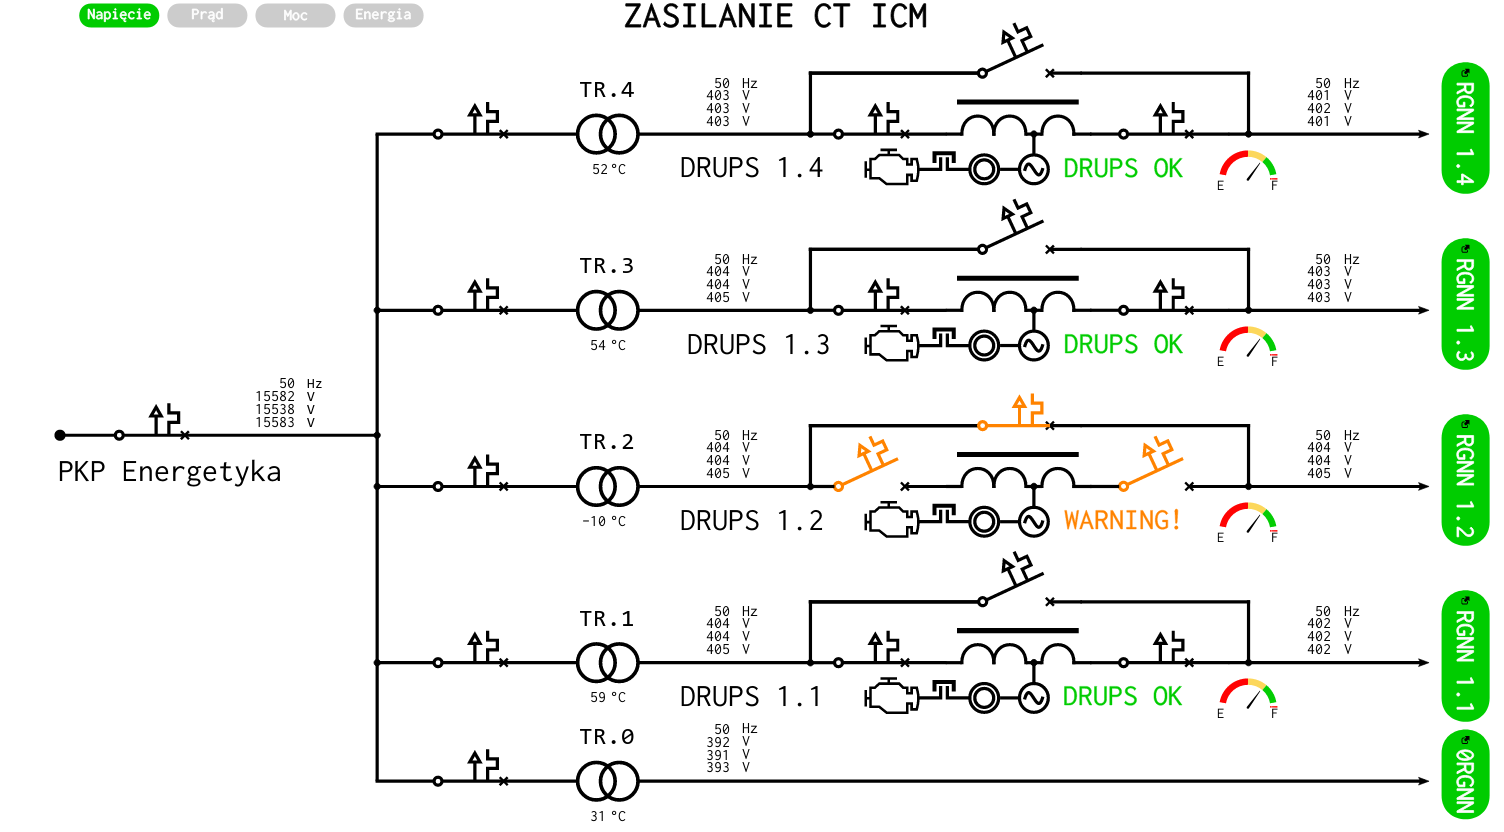
\includegraphics[width=.8\textwidth]{monitoring_obiektow_data_center-img/monitoring_dc-zasilanie}\end{center}
\end{frame}

\subsection{Wizualizacja - detekcja wycieku}
\begin{frame}[fragile]
\begin{center}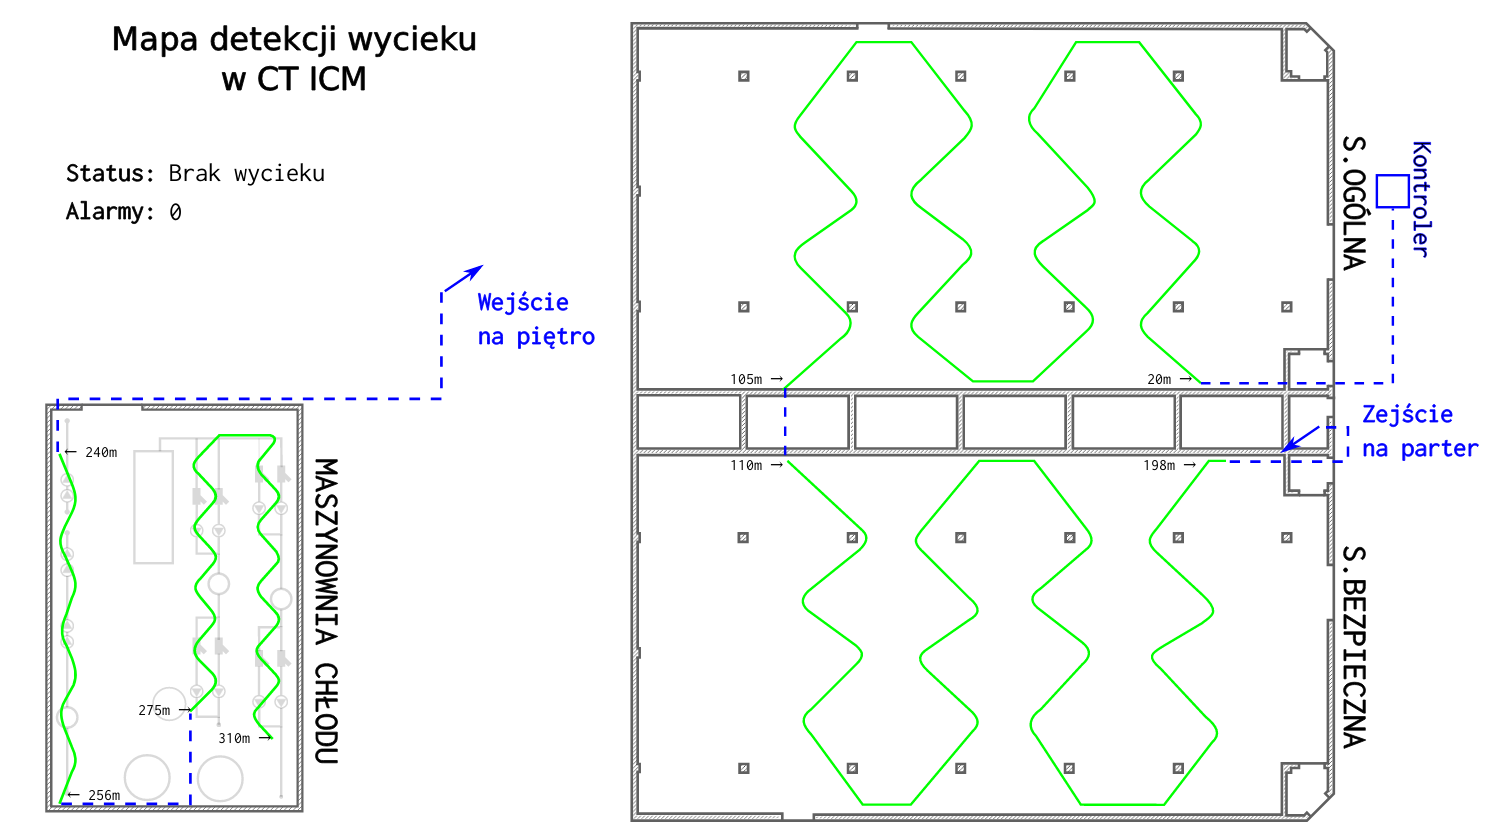
\includegraphics[width=.8\textwidth]{monitoring_obiektow_data_center-img/monitoring_dc-detekcja_wycieku}\\
{\small System detekcji wycieku z (odbiciową) identyfikacją miejsca na którym wystąpił wyciek.}\end{center}
\end{frame}

\subsection{Wizualizacja - system sygnalizacji pożaru}
\begin{frame}[fragile]
\begin{center}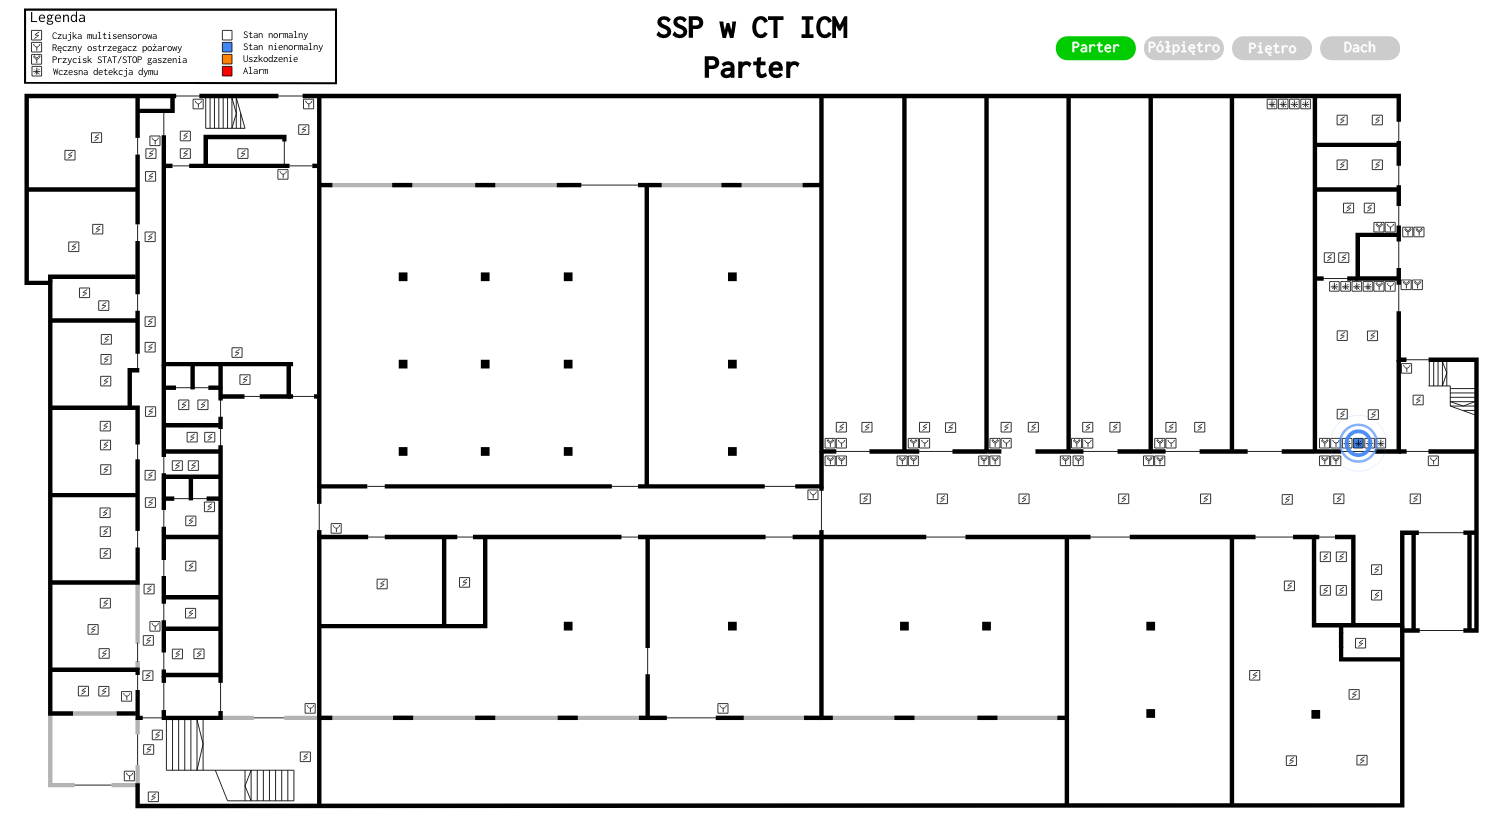
\includegraphics[width=.8\textwidth]{monitoring_obiektow_data_center-img/monitoring_dc-ssp}\end{center}
\end{frame}

\subsection{Wizualizacja - obieg chłodniczy z odzyskiem ciepła}
\begin{frame}[fragile]
\begin{center}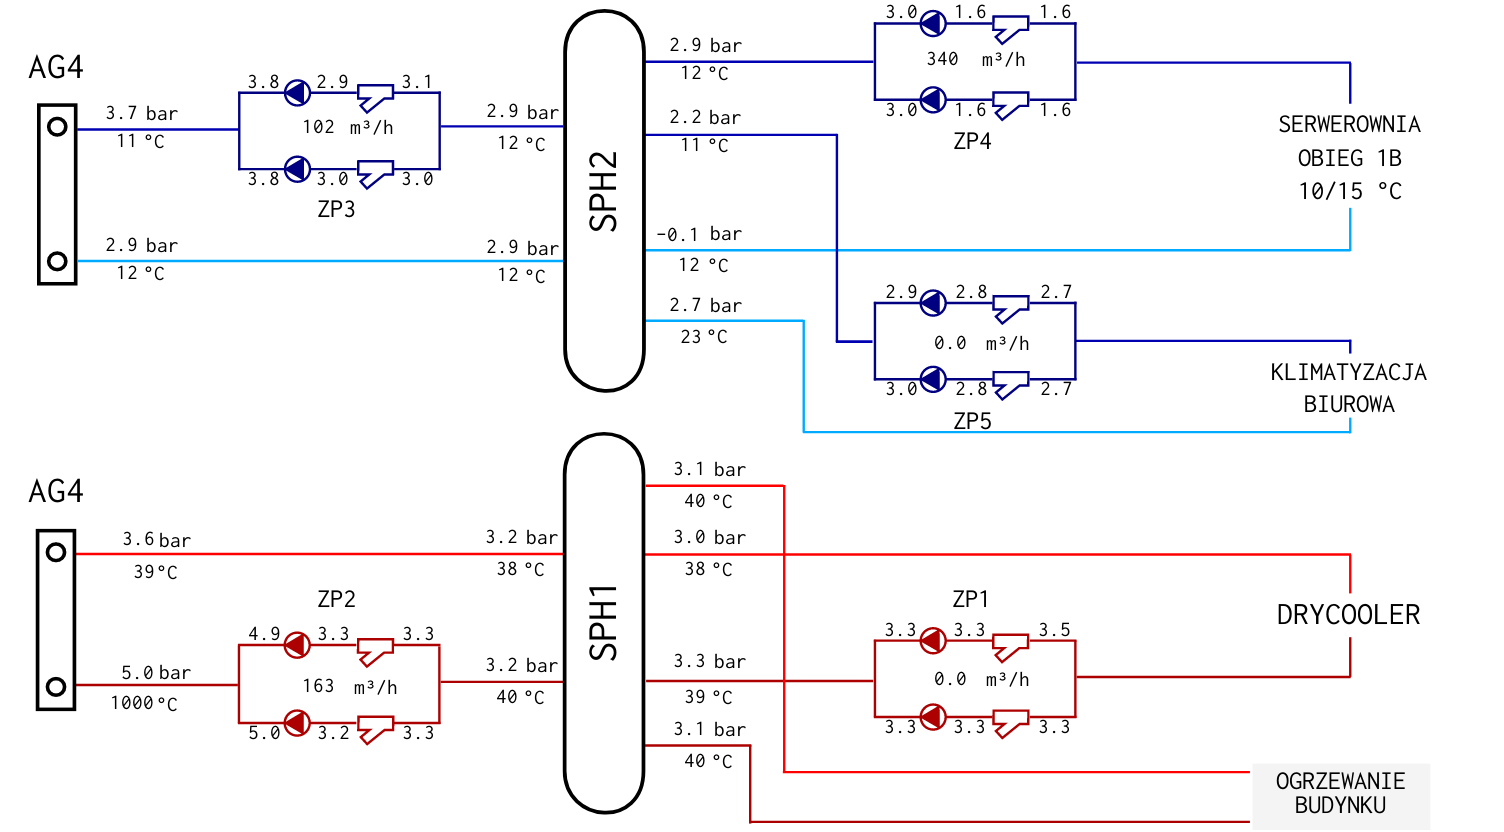
\includegraphics[width=.8\textwidth]{monitoring_obiektow_data_center-img/monitoring_dc-chlodzenie1}\end{center}
\end{frame}

\subsection{Wizualizacja - obieg chłodniczy z freecoolingiem}
\begin{frame}[fragile]
\begin{center}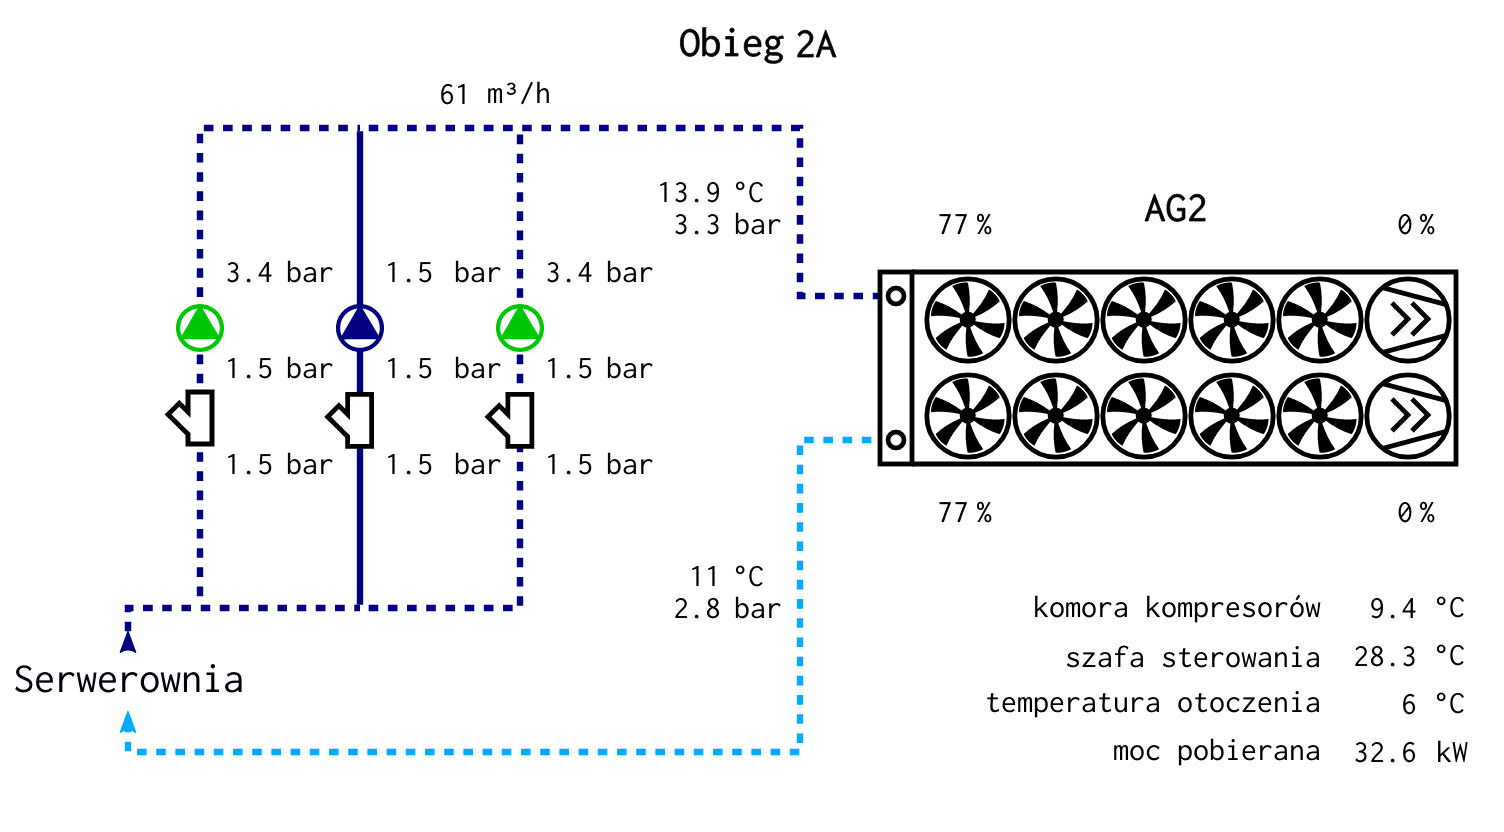
\includegraphics[width=.8\textwidth]{monitoring_obiektow_data_center-img/monitoring_dc-chodzenie2}\end{center}
\end{frame}

\subsection{Zabbix - podgląd parametrów}
\begin{frame}[fragile]
\begin{center}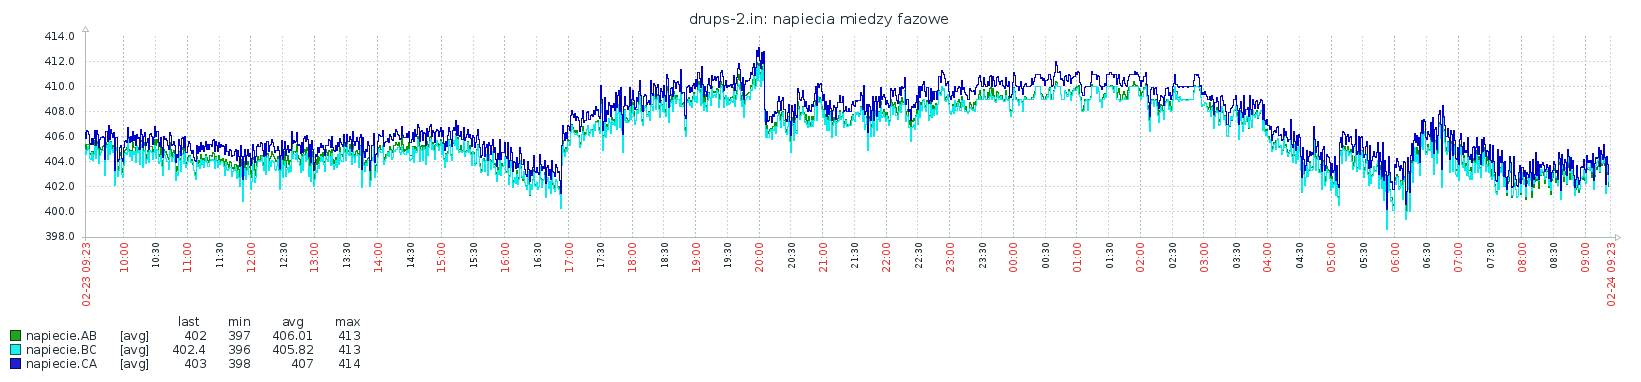
\includegraphics[width=.9\textwidth]{monitoring_obiektow_data_center-img/monitoring_dc-napiecie}\end{center}
\begin{center}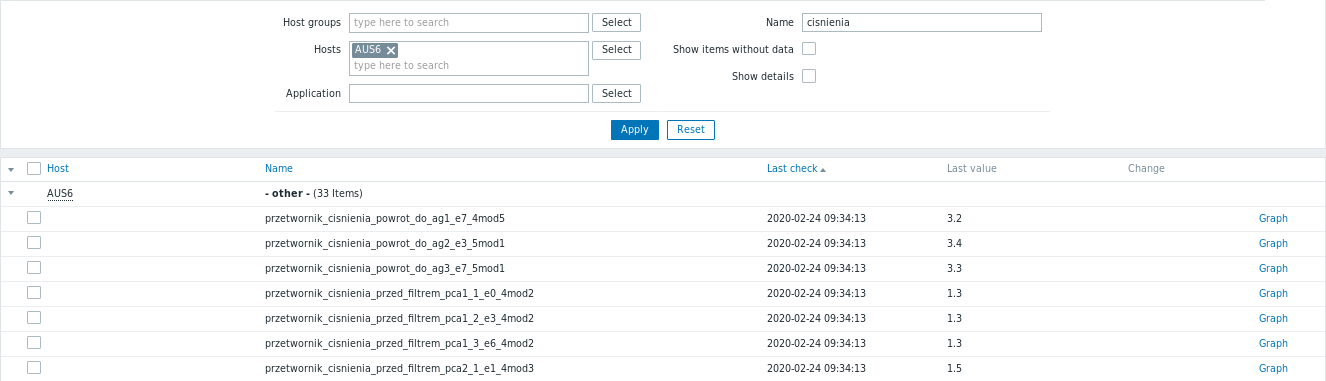
\includegraphics[width=.8\textwidth]{monitoring_obiektow_data_center-img/monitoring_dc-cisnienia}\end{center}
\end{frame}


\section{Pytania?}

\begin{frame}
\begin{center}
\LARGE Pytania?
\end{center}
\end{frame}


\section{Licencja}

\begin{frame}
\small
Copyright © 2020, Robert Ryszard Paciorek <rrp@opcode.eu.org>

Copyright © 2020, Interdyscyplinarne Centrum Modelowania Matematycznego i Komputerowego UW

\footnotesize\vspace{1.5em}
To jest wolny i otwarty dokument. Redystrybucja, użytkowanie i/lub modyfikacja SĄ DOZWOLONE na warunkach licencji MIT.

\vspace{1.5em}
This is free and open document. Redistribution, use and/or modify ARE PERMITTED under the terms of the MIT license.

\tiny\vspace{2em}
Permission is hereby granted, free of charge, to any person obtaining a copy
of this software and associated documentation files (the "Software"), to deal
in the Software without restriction, including without limitation the rights
to use, copy, modify, merge, publish, distribute, sublicense, and/or sell
copies of the Software, and to permit persons to whom the Software is
furnished to do so, subject to the following conditions:

\vspace{1em}
The above copyright notice and this permission notice shall be included in all
copies or substantial portions of the Software.

\vspace{1em}
THE SOFTWARE IS PROVIDED "AS IS", WITHOUT WARRANTY OF ANY KIND, EXPRESS OR
IMPLIED, INCLUDING BUT NOT LIMITED TO THE WARRANTIES OF MERCHANTABILITY,
FITNESS FOR A PARTICULAR PURPOSE AND NONINFRINGEMENT. IN NO EVENT SHALL THE
AUTHORS OR COPYRIGHT HOLDERS BE LIABLE FOR ANY CLAIM, DAMAGES OR OTHER
LIABILITY, WHETHER IN AN ACTION OF CONTRACT, TORT OR OTHERWISE, ARISING FROM,
OUT OF OR IN CONNECTION WITH THE SOFTWARE OR THE USE OR OTHER DEALINGS IN THE
SOFTWARE.

\end{frame}

\end{document}
